
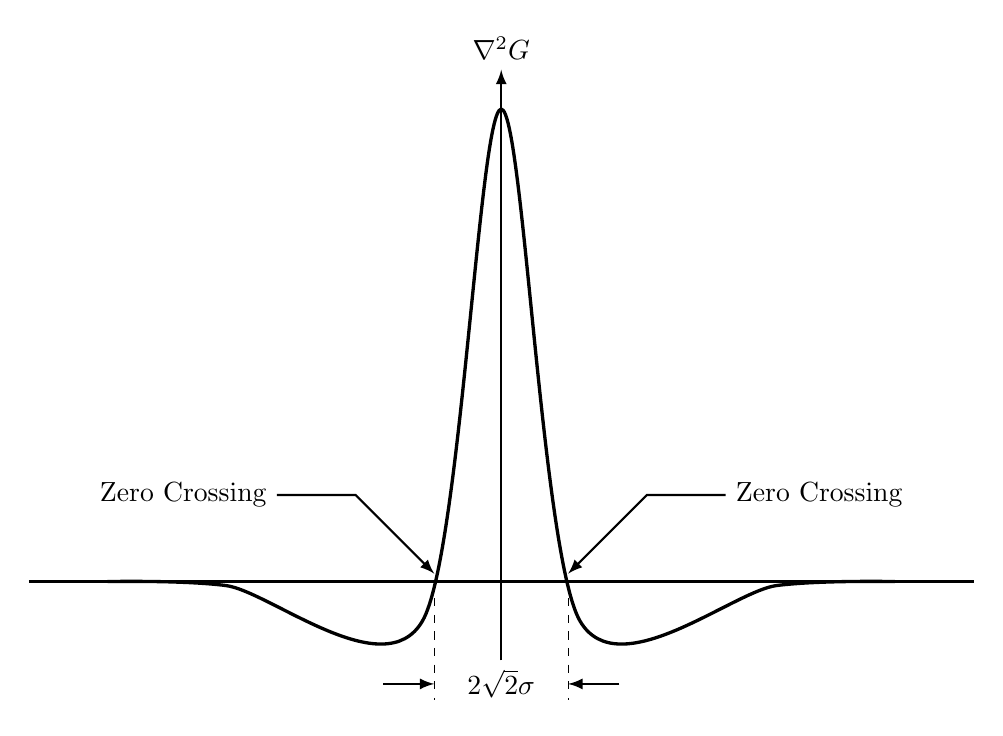
\begin{tikzpicture}
	\draw[thick] (-6,0) -- (6,0);
	\draw[thick, -latex] (0,-1) -- (0, 6.5) node[above] {$\nabla^2G$};
	
	\draw[latex-, thick] (-.85,0.10) -- ++(-1,1) -- ++(-1,0) node[left] {Zero Crossing};
	\draw[latex-, thick] (.85,0.10) -- ++(1,1) -- ++(1,0) node[right] {Zero Crossing};
	
	\draw[dashed] (-.85, 0) -- (-.85, -1.5);
	\draw[dashed] (.85, 0) -- (.85, -1.5);
	\draw (0,-1.3) node {$2\sqrt{2}\sigma$};
	\draw[-latex, thick] (-1.5,-1.3) --(-.85 , -1.3);
	\draw[-latex, thick] (1.5,-1.3) --(.85 , -1.3);	

	\draw[very thick] plot [smooth] coordinates {(-5,0) (-3.5,-0.05) (-1,-0.5) (0,6) (1,-0.5) (3.5,-0.05) (5,0)};
\end{tikzpicture}
